\chapter{Il moto nel piano}

Nel capitolo precedente ci siamo limitati ai corpi che si muovono lungo una \textit{retta}: in quel caso una sola coordinata basta a individuare la posizione, e la velocità cambia soltanto in valore (aumenta o diminuisce). Ma la maggior parte dei moti che vediamo ogni giorno avviene lungo traiettorie \textit{curve}: le pale di un ventilatore, una giostra, un sasso lanciato, la Luna attorno alla Terra.

Per descrivere questi moti servono \textbf{due} coordinate, e occorre trattare la velocità per quello che è davvero: un \textbf{vettore}, con un modulo, una direzione e un verso. In un moto curvo la velocità può cambiare direzione anche quando il suo modulo resta costante -- e vedremo che questo basta a far comparire un'accelerazione.

In questo capitolo studiamo quattro moti curvi importanti (circolare uniforme, armonico, parabolico) e la regola per combinare due moti che avvengono contemporaneamente.

\section{Il moto circolare uniforme}

\subsection{Il vettore velocità}
Finora abbiamo trattato la velocità come uno scalare, occupandoci solo del suo modulo. In un moto rettilineo questo era sufficiente: la direzione del moto è sempre la stessa. In un moto curvo, invece, dobbiamo dire anche \emph{dove punta} la velocità.

\begin{definizione}
In ogni istante il \textbf{vettore velocità} di un punto materiale ha:
\begin{itemize}
    \item \textbf{modulo} uguale alla velocità istantanea;
    \item \textbf{direzione} tangente alla traiettoria nel punto in cui si trova il corpo;
    \item \textbf{verso} concorde con quello di percorrenza della traiettoria.
\end{itemize}
\end{definizione}

Che la velocità sia tangente alla traiettoria si vede bene quando qualcosa si stacca da un moto curvo: le scintille che partono da una mola, il fango che schizza via da una ruota di bicicletta, un martello lanciato dall'atleta partono tutti \emph{lungo la tangente}, non lungo il raggio.

\begin{figure}[!htbp]
    \centering
    \begin{tikzpicture}[>=stealth]
        % traiettoria: parabola y = -0.16 x^2 + 0.45 x  (derivata: -0.32 x + 0.45)
        \draw[ocre,very thick,samples=100,domain=-2.7:4.2,smooth]
            plot ({\x},{-0.16*\x*\x + 0.45*\x});
        \foreach \px/\lab/\lpos in {-2/A/{below}, 1.1/B/{above}, 3.4/C/{below right}}{
            \pgfmathsetmacro\py{-0.16*\px*\px + 0.45*\px}
            \pgfmathsetmacro\slope{-0.32*\px + 0.45}
            \pgfmathsetmacro\nn{sqrt(1 + \slope*\slope)}
            \pgfmathsetmacro\ux{1.4/\nn}
            \pgfmathsetmacro\uy{1.4*\slope/\nn}
            \fill (\px,\py) circle (2pt) node[\lpos]{$\lab$};
            \draw[->,very thick,blue!60!black] (\px,\py) -- ++(\ux,\uy)
                node[anchor=south west,inner sep=1pt]{$\vec v_{\lab}$};
        }
    \end{tikzpicture}
    \caption{In un moto qualsiasi il vettore velocità è, istante per istante, tangente alla traiettoria. Il suo modulo e la sua direzione possono cambiare da punto a punto.}
    \label{fig:v-tangente}
\end{figure}

\subsection{Traiettoria circolare e velocità costante in modulo}
Un punto materiale si muove di \textbf{moto circolare} quando la sua traiettoria è una circonferenza. Se, inoltre, il modulo della velocità resta sempre lo stesso, il moto si dice \textbf{circolare uniforme}.

\begin{definizione}
Il \textbf{moto circolare uniforme} è il moto di un punto lungo una circonferenza, percorsa con velocità di \textbf{modulo costante}. Il vettore velocità ha sempre lo stesso modulo, ma cambia continuamente direzione, restando tangente alla circonferenza.
\end{definizione}

In un moto circolare uniforme il punto percorre archi uguali in intervalli di tempo uguali. In particolare impiega sempre lo stesso tempo a compiere un giro completo.

\begin{definizione}
Si chiama \textbf{periodo} $T$ il tempo impiegato dal punto a percorrere un'intera circonferenza. Si misura in secondi.
\end{definizione}

Poiché in un giro il punto percorre la lunghezza della circonferenza, $2\pi r$, in un tempo $T$, il modulo della sua velocità è

\[ \colorboxed{ocre}{ v = \frac{2\pi r}{T}. } \]

\begin{figure}[!htbp]
    \centering
    \begin{tikzpicture}[>=stealth]
        \draw[gray!70] (0,0) circle (2);
        \fill (0,0) circle (1.3pt) node[below right]{$O$};
        \draw[gray,dashed] (0,0) -- (35:2) node[midway,above,black]{$r$};
        \foreach \a in {0,45,...,315}{
            \fill (\a:2) circle (1.6pt);
            \draw[->,very thick,ocre] (\a:2) -- ++({\a+90}:1.1);
        }
        \node[ocre] at (0,2.9) {$\vec v$};
        \node[ocre] at (2.9,0) {$\vec v$};
    \end{tikzpicture}
    \caption{Moto circolare uniforme: il vettore velocità ha modulo costante e in ogni punto è tangente alla circonferenza (perpendicolare al raggio).}
    \label{fig:mcu-v}
\end{figure}

\begin{testexample}[\thetcbcounter \, Un trenino su una pista circolare]
Un trenino elettrico percorre una pista circolare di raggio $r = \SI{2,50}{\metre}$ compiendo un giro completo in $T = \SI{10,0}{\second}$. Qual è il modulo della sua velocità?
\[ v = \frac{2\pi r}{T} = \frac{2\pi \cdot \SI{2,50}{\metre}}{\SI{10,0}{\second}} \approx \SI{1,57}{\metre\per\second}. \]
\end{testexample}

\begin{testexample}[\thetcbcounter \, Un cavallo della giostra]
Su una giostra un cavallo si trova a $r = \SI{4,0}{\metre}$ dall'asse e compie un giro ogni $T = \SI{8,0}{\second}$. Che velocità ha?
\[ v = \frac{2\pi r}{T} = \frac{2\pi \cdot \SI{4,0}{\metre}}{\SI{8,0}{\second}} \approx \SI{3,1}{\metre\per\second} \approx \SI{11}{\kilo\metre\per\hour}. \]
Un cavallo montato più vicino al centro, sulla stessa giostra, impiega lo stesso tempo $T$ a fare il giro, ma percorre una circonferenza più piccola: la sua velocità è minore.
\end{testexample}

\subsection{Il periodo e la frequenza}
Per i moti che si ripetono molte volte al secondo (un disco che gira, un motore) è più comodo indicare \emph{quanti giri} si compiono nell'unità di tempo, invece del tempo di un singolo giro.

\begin{definizione}
Si chiama \textbf{frequenza} $f$ il numero di giri compiuti nell'unità di tempo. Nel Sistema Internazionale si misura in \textbf{hertz} (\si{\hertz}): $\SI{1}{\hertz}$ è un giro al secondo.
\end{definizione}

Periodo e frequenza sono legati da una relazione semplice: se un giro dura $T$ secondi, in un secondo se ne compiono $1/T$. Quindi

\[ \colorboxed{ocre}{ f = \frac{1}{T}, \qquad T = \frac{1}{f}. } \]

La frequenza è il \textbf{reciproco} del periodo. Nella pratica si incontra spesso anche la frequenza espressa in \textbf{giri al minuto} (in inglese \emph{rpm}, \emph{revolutions per minute}): per passare ai \si{\hertz} si divide per \num{60}.

Sostituendo $T = 1/f$ nella formula della velocità si ottiene un'altra espressione utile:
\[ v = \frac{2\pi r}{T} = 2\pi r\,f. \]

\begin{testexample}[\thetcbcounter \, Il disco rigido di un computer]
Il disco di un vecchio computer gira a \SI{5400}{} giri al minuto. Qual è la sua frequenza in \si{\hertz}? E il periodo?

La frequenza è
\[ f = \frac{5400}{\SI{60}{\second}} = \SI{90}{\hertz}, \]
cioè il disco compie \num{90} giri al secondo. Il periodo è
\[ T = \frac{1}{f} = \frac{1}{\SI{90}{\hertz}} \approx \SI{0,011}{\second} = \SI{11}{\milli\second}. \]
\end{testexample}

\begin{testexample}[\thetcbcounter \, La lancetta dei secondi]
La punta della lancetta dei secondi di un orologio dista $r = \SI{8,0}{\milli\metre}$ dal centro. Calcoliamo periodo, frequenza e velocità della punta.

La lancetta compie un giro in un minuto, quindi $T = \SI{60}{\second}$ e
\[ f = \frac{1}{T} = \frac{1}{\SI{60}{\second}} \approx \SI{0,017}{\hertz}. \]
La velocità della punta è
\[ v = \frac{2\pi r}{T} = \frac{2\pi \cdot \SI{8,0e-3}{\metre}}{\SI{60}{\second}} \approx \SI{8,4e-4}{\metre\per\second}, \]
cioè meno di un millimetro al secondo.
\end{testexample}

\subsection{L'accelerazione centripeta}
In un moto circolare uniforme il modulo della velocità non cambia. Verrebbe da dire che l'accelerazione è nulla. \textbf{Non è così}: l'accelerazione misura la variazione del \emph{vettore} velocità, e in questo moto il vettore velocità cambia di continuo \emph{direzione}. C'è quindi un'accelerazione, anche se la ``fretta'' del corpo non aumenta mai.

Per capire dove punta, consideriamo il corpo in due istanti vicini, in cui ha velocità $\vec v_1$ e $\vec v_2$ (stesso modulo, direzioni diverse). La variazione di velocità è il vettore $\Delta\vec v = \vec v_2 - \vec v_1$, che si costruisce con il metodo punta-coda (figura~\ref{fig:centripeta}). Si vede che, quando i due istanti sono molto vicini, $\Delta\vec v$ è diretto \textbf{verso il centro} della circonferenza. Lo stesso vale allora per l'accelerazione $\vec a = \Delta\vec v / \Delta t$.

\begin{definizione}
In un moto circolare uniforme è sempre presente un'\textbf{accelerazione centripeta} $a_c$, diretta verso il centro della circonferenza, di modulo
\[ \colorboxed{ocre}{ a_c = \frac{v^2}{r}, } \]
dove $v$ è il modulo della velocità e $r$ il raggio.
\end{definizione}

\begin{figure}[!htbp]
    \centering
    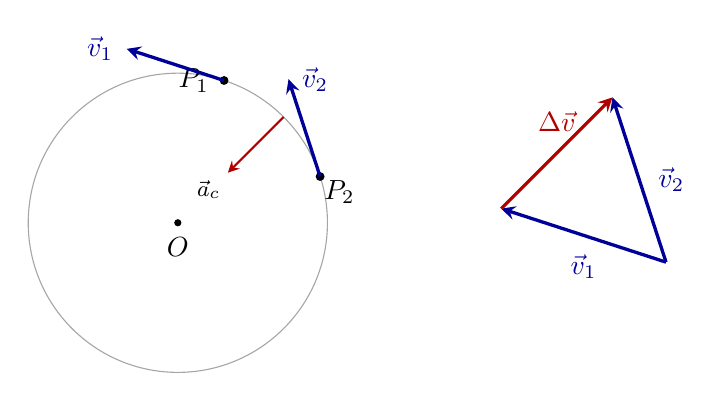
\begin{tikzpicture}[>=stealth,scale=1]
        \draw[gray!70] (0,0) circle (1.9);
        \fill (0,0) circle (1.3pt) node[below=2pt]{$O$};
        % due posizioni vicine: tangente = raggio + 90 gradi
        \coordinate (P1) at (72:1.9);
        \coordinate (P2) at (18:1.9);
        \fill (P1) circle (1.6pt) node[left=2pt]{$P_1$};
        \fill (P2) circle (1.6pt) node[below right=-2pt]{$P_2$};
        \draw[->,very thick,blue!60!black] (P1) -- ++(162:1.3) node[left=1pt]{$\vec v_1$};
        \draw[->,very thick,blue!60!black] (P2) -- ++(108:1.3) node[right=1pt]{$\vec v_2$};
        \draw[->,thick,red!70!black] (45:1.9) -- (45:0.9) node[below left=-1pt,black]{\footnotesize $\vec a_c$};
        % costruzione Delta v = v2 - v1, ingrandita a lato, etichette fuori dal triangolo
        \begin{scope}[shift={(6.2,-0.5)}]
            \draw[->,very thick,blue!60!black] (0,0) -- (162:2.2)
                node[midway,below=3pt]{$\vec v_1$};
            \draw[->,very thick,blue!60!black] (0,0) -- (108:2.2)
                node[pos=0.5,right=3pt]{$\vec v_2$};
            \draw[->,very thick,red!70!black] (162:2.2) -- (108:2.2)
                node[midway,above=4pt]{$\Delta\vec v$};
        \end{scope}
    \end{tikzpicture}
    \caption{Costruzione di $\Delta\vec v = \vec v_2 - \vec v_1$ per due posizioni vicine. Quando $\Delta t$ è piccolo, $\Delta\vec v$ (e quindi l'accelerazione) punta verso il centro: è l'accelerazione centripeta.}
    \label{fig:centripeta}
\end{figure}

\begin{remark}
L'accelerazione centripeta non fa aumentare la velocità: la sua funzione è solo quella di ``curvare'' continuamente la traiettoria, cambiando la direzione di $\vec v$ senza toccarne il modulo. È l'effetto che sentiamo come spinta verso l'esterno in un'auto che affronta una curva stretta: in realtà è il sedile che ci spinge verso il centro della curva, imprimendoci l'accelerazione centripeta.
\end{remark}

\begin{testexample}[\thetcbcounter \, L'accelerazione centripeta del trenino]
Riprendiamo il trenino dell'esempio precedente: $r = \SI{2,50}{\metre}$, $v \approx \SI{1,57}{\metre\per\second}$. L'accelerazione centripeta vale
\[ a_c = \frac{v^2}{r} = \frac{(\SI{1,57}{\metre\per\second})^2}{\SI{2,50}{\metre}} \approx \SI{0,99}{\metre\per\second\squared}, \]
diretta in ogni istante verso il centro della pista.
\end{testexample}

\begin{esercizio}
Un'automobilina su una pista circolare di raggio \SI{25}{\centi\metre} compie un giro in \SI{1,0}{\second}. Calcola il modulo della sua velocità e l'accelerazione centripeta.\\
\risp{$v \approx \SI{1,57}{\metre\per\second}$; \; $a_c \approx \SI{9,9}{\metre\per\second\squared}$}
\end{esercizio}

\begin{esercizio}
L'elica di un aereo compie \SI{2400}{} giri al minuto. Trasforma la frequenza in \si{\hertz} e calcola il periodo di rotazione.\\
\risp{$f = \SI{40}{\hertz}$; \; $T = \SI{0,025}{\second}$}
\end{esercizio}

\begin{esercizio}
La ruota di una bicicletta ha diametro \SI{60}{\centi\metre}. Un tassello del battistrada si muove alla velocità di \SI{36}{\kilo\metre\per\hour}. Quanto tempo impiega a compiere un giro completo?\\
\risp{$T = \dfrac{2\pi r}{v} \approx \SI{0,19}{\second}$}
\end{esercizio}

\begin{esercizio}
Un sasso è legato a una corda lunga \SI{0,80}{\metre} e fatto ruotare in un piano orizzontale con frequenza \SI{2,0}{\hertz}. Calcola la velocità del sasso e la sua accelerazione centripeta.\\
\risp{$v \approx \SI{10,1}{\metre\per\second}$; \; $a_c \approx \SI{126}{\metre\per\second\squared}$}
\end{esercizio}

\begin{esercizio}
Il cestello di una lavatrice ha diametro \SI{40}{\centi\metre} e nella centrifuga compie \SI{1200}{} giri al minuto. Qual è la frequenza in \si{\hertz}? A quale accelerazione centripeta è sottoposta la biancheria a contatto con la parete?\\
\risp{$f = \SI{20}{\hertz}$; \; $a_c \approx \SI{3,2e3}{\metre\per\second\squared}$}
\end{esercizio}

\begin{esercizio}
La Terra percorre attorno al Sole un'orbita quasi circolare di raggio \SI{1,5e11}{\metre} in un anno ($T \approx \SI{3,15e7}{\second}$). Verifica che la sua velocità è circa \SI{30}{\kilo\metre\per\second} e calcola l'accelerazione centripeta.\\
\risp{$v \approx \SI{2,99e4}{\metre\per\second}$; \; $a_c \approx \SI{5,9e-3}{\metre\per\second\squared}$}
\end{esercizio}

\section{La velocità angolare}

Nel moto circolare, mentre il punto percorre un arco, il raggio che lo congiunge al centro descrive un \textbf{angolo}. Possiamo allora descrivere il moto in un modo nuovo: non seguendo lo spazio percorso lungo la circonferenza, ma l'angolo ``spazzato'' dal raggio. È spesso più comodo, perché l'angolo non dipende da quanto è grande la circonferenza.

\subsection{La misura degli angoli: il radiante}
Nella vita di tutti i giorni gli angoli si misurano in \textbf{gradi} (un giro completo vale $360^\circ $). In fisica, però, conviene un'altra unità, il \textbf{radiante}, legata direttamente alla circonferenza.

\begin{definizione}
L'ampiezza di un angolo \textbf{in radianti} è il rapporto fra la lunghezza dell'arco che esso sottende e il raggio della circonferenza:
\[ \colorboxed{ocre}{ \alpha = \frac{\text{arco}}{\text{raggio}} = \frac{\ell}{r}. } \]
Essendo il rapporto fra due lunghezze, l'angolo in radianti è un \textbf{numero puro} (l'unità \si{\radian} si può omettere nei calcoli).
\end{definizione}

Un angolo di \textbf{1 radiante} è quello che sottende un arco lungo quanto il raggio (figura~\ref{fig:radiante}). Poiché l'intera circonferenza è lunga $2\pi r$, l'angolo giro vale
\[ \alpha_{\text{giro}} = \frac{2\pi r}{r} = 2\pi \ \si{\radian}, \]
cioè $360^\circ  = 2\pi\ \si{\radian}$. Da qui
\[ \SI{1}{\radian} = \frac{360^\circ }{2\pi} \approx 57,3^\circ . \]
Per convertire un angolo da gradi ($\alpha_g$) a radianti ($\alpha_r$), o viceversa, si usa la proporzione
\[ \alpha_r : \pi = \alpha_g : 180^\circ . \]

\begin{figure}[!htbp]
    \centering
    \begin{tikzpicture}[>=stealth,scale=1.1]
        \draw[gray!70] (0,0) circle (2);
        \fill (0,0) circle (1.2pt) node[below left]{$O$};
        \draw[thick] (0,0) -- (0:2) node[midway,below]{$r$};
        \draw[thick] (0,0) -- (57.3:2);
        \node[above] at (57.3:1) {$r$};
        \draw[ocre,very thick] (0:2) arc (0:57.3:2);
        \node[ocre,right] at (28:2.35) {$\ell = r$};
        \draw (0:0.55) arc (0:57.3:0.55);
        \node at (28:0.85) {\footnotesize $1\ \si{\radian}$};
    \end{tikzpicture}
    \caption{Un radiante è l'angolo al centro che sottende un arco $\ell$ lungo quanto il raggio $r$.}
    \label{fig:radiante}
\end{figure}

\begin{testexample}[\thetcbcounter \, Da gradi a radianti e viceversa]
Convertiamo $60^\circ $ in radianti:
\[ \alpha_r = \frac{\pi \cdot 60^\circ }{180^\circ } = \frac{\pi}{3} \approx \SI{1,05}{\radian}. \]
Convertiamo ora \SI{2,0}{\radian} in gradi:
\[ \alpha_g = \frac{180^\circ  \cdot 2,0}{\pi} \approx 114,6^\circ . \]
\end{testexample}

\subsection{La velocità angolare}
Se un punto si muove lungo una circonferenza, il raggio che lo congiunge al centro descrive un angolo $\alpha$ tanto maggiore quanto più veloce è il moto. Possiamo allora misurare la rapidità del moto guardando l'angolo, invece dell'arco.

\begin{definizione}
La \textbf{velocità angolare} $\omega$ (lettera greca ``òmega'') è il rapporto fra l'angolo descritto dal raggio e l'intervallo di tempo impiegato a descriverlo:
\[ \colorboxed{ocre}{ \omega = \frac{\Delta\alpha}{\Delta t}. } \]
Si misura in \textbf{radianti al secondo} (\si{\radian\per\second}).
\end{definizione}

\begin{testexample}[\thetcbcounter \, Un quarto di giro]
Un punto descrive un angolo di $90^\circ $ (cioè $\pi/2$ radianti) in \SI{4,0}{\second}. La sua velocità angolare media è
\[ \omega = \frac{\Delta\alpha}{\Delta t} = \frac{\pi/2\ \si{\radian}}{\SI{4,0}{\second}} \approx \SI{0,39}{\radian\per\second}. \]
\end{testexample}

\subsection{La velocità angolare nel moto circolare uniforme}
Se il moto è circolare uniforme, in un periodo $T$ il raggio descrive un angolo giro, $2\pi$ radianti. La velocità angolare è quindi costante e vale
\[ \colorboxed{ocre}{ \omega = \frac{2\pi}{T} = 2\pi f. } \]

\subsection{Le relazioni fra \texorpdfstring{$v$}{v}, \texorpdfstring{$\omega$}{omega} e \texorpdfstring{$a_c$}{ac}}
La velocità lungo la traiettoria, che d'ora in poi chiamiamo \textbf{velocità tangenziale} $v$ (perché è tangente alla circonferenza), è legata alla velocità angolare in modo semplice. Partiamo da $v = 2\pi r / T$ e sostituiamo $2\pi/T = \omega$:
\[ \colorboxed{ocre}{ v = \omega\,r. } \]
La velocità tangenziale è direttamente proporzionale al raggio: a parità di $\omega$, un punto più lontano dal centro si muove più in fretta.

Sostituendo $v = \omega r$ nell'accelerazione centripeta $a_c = v^2/r$ si ottiene una seconda espressione:
\[ a_c = \frac{(\omega r)^2}{r} = \omega^2\,r. \]

\begin{remark}
In un corpo rigido che ruota attorno a un asse (un disco, una giostra, la Terra), \textbf{tutti i punti hanno la stessa velocità angolare} $\omega$: compiono un giro nello stesso tempo. La velocità tangenziale $v = \omega r$, invece, \textbf{è diversa da punto a punto}: cresce allontanandosi dall'asse. Per questo il bordo di una mola si muove molto più velocemente di un punto vicino al centro, pur girando ``insieme''.
\end{remark}

\begin{testexample}[\thetcbcounter \, Due punti di una piattaforma rotante]
Una piattaforma gira con periodo $T = \SI{0,10}{\second}$. Il punto $A$ dista \SI{10}{\centi\metre} dall'asse, il punto $B$ ne dista \SI{20}{\centi\metre}. Calcoliamo velocità angolari e velocità tangenziali.

La velocità angolare è la stessa per i due punti:
\[ \omega_A = \omega_B = \frac{2\pi}{T} = \frac{2\pi}{\SI{0,10}{\second}} \approx \SI{63}{\radian\per\second}. \]
Le velocità tangenziali, invece, dipendono dal raggio:
\[ v_A = \omega\,r_A \approx 62,8 \cdot \SI{0,10}{\metre} \approx \SI{6,3}{\metre\per\second}, \qquad v_B = \omega\,r_B \approx 62,8 \cdot \SI{0,20}{\metre} \approx \SI{13}{\metre\per\second}. \]
Il punto $B$, con raggio doppio, ha velocità tangenziale doppia.
\end{testexample}

\begin{figure}[!htbp]
    \centering
    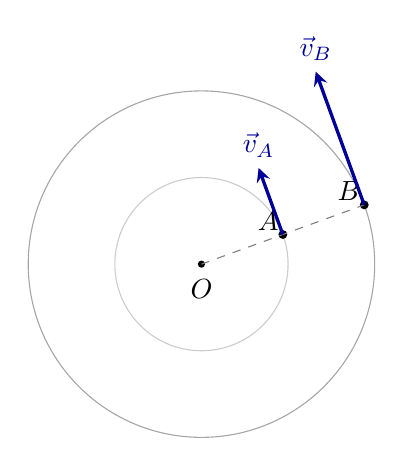
\begin{tikzpicture}[>=stealth]
        \draw[gray!70] (0,0) circle (2.2);
        \draw[gray!40] (0,0) circle (1.1);
        \fill (0,0) circle (1.3pt) node[below=2pt]{$O$};
        \fill (20:1.1) circle (1.6pt) node[above left=-2pt]{$A$};
        \fill (20:2.2) circle (1.6pt) node[above left=-2pt]{$B$};
        \draw[gray,dashed] (0,0) -- (20:2.2);
        \draw[->,very thick,blue!60!black] (20:1.1) -- ++(110:0.9) node[above]{$\vec v_A$};
        \draw[->,very thick,blue!60!black] (20:2.2) -- ++(110:1.8) node[above]{$\vec v_B$};
    \end{tikzpicture}
    \caption{In un corpo rigido rotante $A$ e $B$ hanno la stessa velocità angolare, ma $B$ (più lontano dall'asse) ha velocità tangenziale maggiore.}
    \label{fig:corpo-rigido}
\end{figure}

\begin{esercizio}
Converti in radianti gli angoli $30^\circ $, $45^\circ $ e $120^\circ $. Converti in gradi l'angolo \SI{1,5}{\radian}.\\
\risp{$\pi/6 \approx 0,52$; \; $\pi/4 \approx 0,79$; \; $2\pi/3 \approx 2,09$ (rad); \quad $\SI{1,5}{\radian} \approx 85,9^\circ $}
\end{esercizio}

\begin{esercizio}
Un motore elettrico gira a \SI{1500}{} giri al minuto (rpm). Calcola la sua velocità angolare in \si{\radian\per\second}.\\
\risp{$\omega \approx \SI{157}{\radian\per\second}$}
\end{esercizio}

\begin{esercizio}
Una giostra compie un giro in \SI{12}{\second}. Calcola la velocità angolare. Un bambino è seduto a \SI{3,5}{\metre} dall'asse: quanto vale la sua velocità tangenziale?\\
\risp{$\omega \approx \SI{0,52}{\radian\per\second}$; \; $v \approx \SI{1,8}{\metre\per\second}$}
\end{esercizio}

\begin{esercizio}
Un disco ha raggio \SI{20}{\centi\metre}. Qual è la massima velocità angolare a cui può girare affinché l'accelerazione centripeta al bordo non superi il valore $g = \SI{9,81}{\metre\per\second\squared}$?\\
\risp{$\omega = \sqrt{g/r} \approx \SI{7,0}{\radian\per\second}$}
\end{esercizio}

\begin{esercizio}
Un satellite orbita attorno alla Terra a un'altezza tale che il raggio dell'orbita è \SI{7,0e6}{\metre}, e compie un giro in \SI{2,0}{\hour}. Calcola periodo in secondi, velocità angolare e velocità del satellite.\\
\risp{$T = \SI{7200}{\second}$; \; $\omega \approx \SI{8,7e-4}{\radian\per\second}$; \; $v \approx \SI{6,1e3}{\metre\per\second}$}
\end{esercizio}

\begin{esercizio}
Le pale di un elicottero sono lunghe \SI{3,0}{\metre} e ruotano con frequenza di \SI{540}{} giri al minuto. Calcola la velocità angolare e la velocità dell'estremo di una pala.\\
\risp{$\omega \approx \SI{56,5}{\radian\per\second}$; \; $v \approx \SI{170}{\metre\per\second}$}
\end{esercizio}

\section{Il moto armonico}

\subsection{La proiezione del moto circolare sul diametro}
Se osserviamo di lato una giostra che gira, un cavallo non ci sembra più muoversi lungo una circonferenza, ma avanti e indietro lungo un segmento. Diamo un significato preciso a questa osservazione.

Consideriamo un punto $P$ che si muove di moto circolare uniforme su una circonferenza di raggio $r$, e indichiamo con $Q$ la sua \textbf{proiezione} su un diametro $AB$ (il piede della perpendicolare calata da $P$ sul diametro). Mentre $P$ gira, $Q$ va avanti e indietro fra $A$ e $B$.

Il moto di $Q$ \textbf{non è uniforme}: quando $P$ è vicino ad $A$ o a $B$, la sua proiezione $Q$ si sposta poco; quando $P$ passa vicino al centro, $Q$ corre. In tempi uguali $Q$ percorre segmenti diversi.

\begin{definizione}
Il moto della proiezione $Q$ su un diametro di un punto $P$ che si muove di moto circolare uniforme si chiama \textbf{moto armonico}.
\begin{itemize}
    \item il \textbf{centro di oscillazione} è il centro della circonferenza;
    \item l'\textbf{ampiezza} $A$ dell'oscillazione è uguale al raggio $r$;
    \item il \textbf{periodo} del moto armonico è uguale a quello del moto circolare che lo genera.
\end{itemize}
\end{definizione}

\begin{figure}[!htbp]
    \centering
    \begin{tikzpicture}[>=stealth,scale=1.2]
        \draw[gray!70] (0,0) circle (1.8);
        \draw[thick] (-1.8,0) -- (1.8,0);
        \node[left] at (-1.8,0) {$B$};
        \node[right] at (1.8,0) {$A$};
        \fill (0,0) circle (1.1pt) node[below left]{$O$};
        \def\a{52}
        \coordinate (P) at (\a:1.8);
        \coordinate (Q) at ({1.8*cos(\a)},0);
        \pgfmathsetmacro\qx{1.8*cos(\a)}
        \draw[thick] (0,0) -- (P) node[midway,above left]{$r$};
        \draw[gray,dashed] (P) -- (Q);
        % il cateto OQ, orizzontale, sul diametro
        \draw[very thick,blue!60!black] (0,0) -- (Q);
        \fill[ocre] (P) circle (1.8pt) node[above right]{$P$};
        \fill[blue!60!black] (Q) circle (1.8pt) node[above=2pt]{$Q$};
        \draw (0.4,0) arc (0:\a:0.4);
        \node at (\a/2:0.62) {\footnotesize $\alpha$};
        \draw[<->,blue!60!black] (0,-0.32) -- (\qx,-0.32)
            node[midway,fill=white,inner sep=1pt]{\footnotesize $s = OQ$};
    \end{tikzpicture}
    \caption{La proiezione $Q$ del punto $P$ sul diametro $AB$ si muove di moto armonico. Nel triangolo rettangolo $OQP$ il cateto $OQ = s$ è adiacente all'angolo $\alpha$, quindi $s = r\cos\alpha$.}
    \label{fig:armonico-proiezione}
\end{figure}

\subsection{La legge oraria del moto armonico}
Vogliamo la posizione $s$ di $Q$ (misurata dal centro $O$) a ogni istante $t$. Supponiamo che a $t = 0$ il punto $P$ si trovi in $A$; al tempo $t$ ha descritto l'angolo $\alpha$. Nel triangolo rettangolo $OQP$ (figura~\ref{fig:armonico-proiezione}) il cateto $OQ$ è adiacente ad $\alpha$, quindi
\[ s = OQ = OP\cos\alpha = r\cos\alpha. \]
Ma il moto di $P$ è circolare uniforme, quindi $\alpha = \omega\,t$. Sostituendo:
\[ \colorboxed{ocre}{ s = A\cos(\omega\,t), } \]
dove $A$ è l'ampiezza (il raggio) e $\omega$ si chiama \textbf{pulsazione} del moto armonico, si misura in \si{\radian\per\second} ed è legata al periodo da $\omega = 2\pi/T$.

\begin{testexample}[\thetcbcounter \, Un peso appeso a una molla]
Un peso attaccato a una molla oscilla su e giù di moto armonico con ampiezza $A = \SI{10}{\centi\metre}$ e velocità angolare $\omega = \SI{1,25}{\radian\per\second}$. Dove si trova dopo $t = \SI{1,0}{\second}$?
\[ s = A\cos(\omega\,t) = \SI{10}{\centi\metre} \cdot \cos(1,25 \cdot 1,0) \approx \SI{10}{\centi\metre} \cdot 0,315 \approx \SI{3,2}{\centi\metre}. \]
Il peso si trova a \SI{3,2}{\centi\metre} dalla posizione di riposo.
\end{testexample}

\subsection{Il grafico spazio--tempo}
Se riportiamo la posizione $s = A\cos(\omega t)$ in funzione del tempo otteniamo una curva chiamata \textbf{cosinusoide} (figura~\ref{fig:cosinusoide}).

\begin{figure}[!htbp]
    \centering
    \begin{tikzpicture}
    \begin{axis}[
        width=0.85\linewidth, height=5.5cm,
        xlabel={$t$}, ylabel={$s$ (cm)},
        x label style={at={(axis description cs:1,-0.04)},anchor=north},
        xmin=0, xmax=8.4, ymin=-13, ymax=13,
        xtick={0,2.1,4.2,6.3,8.4},
        xticklabels={$0$,$\tfrac{T}{4}$,$\tfrac{T}{2}$,$\tfrac{3}{4}T$,$T$},
        ytick={-10,-5,0,5,10},
        grid=both, grid style={gray!20},
    ]
    \addplot[ocre, very thick, samples=100, domain=0:8.4] {10*cos(deg(2*pi*x/8.4))};
    \end{axis}
    \end{tikzpicture}
    \caption{Grafico spazio--tempo di un moto armonico di ampiezza \SI{10}{\centi\metre}: una cosinusoide. La posizione oscilla fra $+A$ e $-A$; il periodo $T$ è il tempo di un'oscillazione completa.}
    \label{fig:cosinusoide}
\end{figure}

Osserviamo alcune proprietà:
\begin{itemize}
    \item la posizione $s$ è sempre compresa fra $+A$ e $-A$;
    \item per $t = 0$, $t = T/2$, $t = T$ il punto è agli estremi dell'oscillazione ($s$ vale $\pm A$);
    \item per $t = T/4$ e $t = 3T/4$ il punto passa per il centro ($s = 0$);
    \item la velocità non è costante: la curva non ha pendenza costante. È massima al centro, nulla agli estremi.
\end{itemize}

Si può dimostrare che nel moto armonico l'accelerazione è
\[ a = -\omega^2\,s. \]

\begin{remark}
L'accelerazione di un moto armonico è \textbf{direttamente proporzionale alla posizione}, ma con segno opposto: quando il punto è spostato verso destra ($s > 0$) l'accelerazione lo richiama verso sinistra, e viceversa. È sempre diretta verso il centro dell'oscillazione. Questo è il ``marchio di fabbrica'' del moto armonico: lo si ritrova ogni volta che una forza di richiamo è proporzionale allo spostamento (una molla che segue la legge di Hooke, un pendolo con piccole oscillazioni).
\end{remark}

\begin{esercizio}
Un moto armonico ha periodo \SI{2,00}{\second}. Qual è la sua pulsazione?\\
\risp{$\omega = \dfrac{2\pi}{T} \approx \SI{3,14}{\radian\per\second}$}
\end{esercizio}

\begin{esercizio}
Un moto armonico ha ampiezza \SI{15}{\centi\metre} e periodo \SI{0,80}{\second}. Calcola la pulsazione $\omega$ e completa la tabella della posizione $s = A\cos(\omega t)$.

\begin{center}
\begin{tabular}{c|ccccc}
    \toprule
    $t$ & $0$ & $T/4$ & $T/2$ & $3T/4$ & $T$ \\[2pt]
    $s$ (cm) & \underline{\hspace{1.1cm}} & \underline{\hspace{1.1cm}} & \underline{\hspace{1.1cm}} & \underline{\hspace{1.1cm}} & \underline{\hspace{1.1cm}} \\
    \bottomrule
\end{tabular}
\end{center}
\risp{$\omega \approx \SI{7,85}{\radian\per\second}$; \quad $s = 15;\ 0;\ -15;\ 0;\ 15$ cm}
\end{esercizio}

\begin{esercizio}
Un punto si muove di moto armonico con ampiezza \SI{8,0}{\centi\metre} e pulsazione \SI{5,0}{\radian\per\second}. Scrivi la legge oraria e calcola la posizione a $t = \SI{0,50}{\second}$.\\
\risp{$s = 8,0\cos(5,0\,t)$ cm; \; a $t = \SI{0,50}{\second}$: $\cos(\SI{2,5}{\radian}) \approx -0,80$, quindi $s \approx \SI{-6,4}{\centi\metre}$ (il punto ha superato il centro)}
\end{esercizio}

\begin{esercizio}
Pizzicando una corda di violino, un suo punto oscilla di moto armonico con frequenza \SI{440}{\hertz} (il ``la''). Qual è la pulsazione del moto? E il periodo?\\
\risp{$\omega = 2\pi f \approx \SI{2765}{\radian\per\second}$; \; $T \approx \SI{2,3e-3}{\second}$}
\end{esercizio}

\begin{esercizio}
Un moto armonico di ampiezza \SI{6,0}{\centi\metre} ha pulsazione \SI{10}{\radian\per\second}. Qual è il modulo massimo dell'accelerazione (raggiunto agli estremi, dove $|s| = A$)?\\
\risp{$a_{\max} = \omega^2 A = \SI{6,0}{\metre\per\second\squared}$}
\end{esercizio}

\section{Il moto parabolico}

\subsection{Il lancio orizzontale}
Consideriamo una biglia che rotola su un tavolo e, arrivata al bordo, prosegue nel vuoto con velocità orizzontale. Da quell'istante è soggetta \emph{contemporaneamente} a due moti indipendenti:
\begin{itemize}
    \item lungo l'\textbf{orizzontale}, un moto rettilineo uniforme: nessuna forza agisce in quella direzione, quindi la velocità orizzontale resta quella con cui la biglia ha lasciato il tavolo;
    \item lungo la \textbf{verticale}, una caduta libera: la biglia parte con velocità verticale nulla e accelera verso il basso con accelerazione $g$.
\end{itemize}

Scegliamo l'origine degli assi nel punto in cui la biglia lascia il tavolo, l'asse $x$ orizzontale nel verso del moto e l'asse $y$ verticale rivolto \textbf{verso il basso}. Con $v_0$ la velocità orizzontale iniziale, le due leggi orarie sono
\[ \colorboxed{ocre}{ x = v_0\,t, \qquad y = \frac{1}{2}\,g\,t^2. } \]
I due moti sono \textbf{indipendenti}: cambiare $v_0$ non modifica la legge della caduta verticale. Una biglia lasciata cadere e una lanciata orizzontalmente dallo stesso tavolo toccano terra \emph{nello stesso istante}.

\begin{figure}[!htbp]
    \centering
    \begin{tikzpicture}[>=stealth,scale=1]
        \draw[->,thick] (0,0) -- (6.3,0) node[right]{$x$};
        \draw[->,thick] (0,0) -- (0,-4.6) node[below]{$y$};
        \fill (0,0) circle (1.3pt) node[above right]{$O$};
        % traiettoria parabolica  y = k x^2, con k tale che a x=5 y=4.2
        \draw[ocre,very thick,samples=60,domain=0:5.4] plot ({\x},{-0.147*\x*\x});
        % posizioni a intervalli di tempo uguali (x = 1,2,3,4,5)
        \foreach \x in {1,...,5}{
            \fill[ocre] (\x,{-0.147*\x*\x}) circle (2pt);
            \draw[gray,dashed] (\x,0) -- (\x,{-0.147*\x*\x});
        }
        \node[ocre,anchor=west] at (5.4,{-0.147*5.4*5.4}) {\footnotesize traiettoria};
        \node[gray] at (3,0.28) {\footnotesize $x = v_0 t$ \; (spazi uguali)};
    \end{tikzpicture}
    \caption{Lancio orizzontale: le posizioni sono segnate a intervalli di tempo uguali. Lungo $x$ gli spazi sono uguali (moto uniforme); lungo $y$ crescono (caduta libera). La traiettoria è una parabola.}
    \label{fig:lancio-orizzontale}
\end{figure}

Ricavando $t = x/v_0$ dalla prima legge e sostituendo nella seconda si trova $y = \dfrac{g}{2v_0^2}\,x^2$: la traiettoria è una \textbf{parabola}. Per questo si parla di \textbf{moto parabolico}.

\begin{testexample}[\thetcbcounter \, Una biglia che lascia il tavolo]
Una biglia lascia un tavolo alto \SI{0,80}{\metre} con velocità orizzontale $v_0 = \SI{2,0}{\metre\per\second}$. Dopo quanto tempo tocca terra? A che distanza dal bordo del tavolo?

Il tempo di caduta dipende \emph{solo} dal moto verticale: la biglia tocca terra quando $y = \SI{0,80}{\metre}$,
\[ 0,80 = \frac{1}{2}\cdot 9{,}81 \cdot t^2 \;\Longrightarrow\; t^2 = \frac{1,60}{9{,}81} \approx 0,163 \;\Longrightarrow\; t \approx \SI{0,40}{\second}. \]
In questo tempo, lungo l'orizzontale, ha percorso
\[ x = v_0\,t \approx 2{,}0 \cdot 0{,}40 \approx \SI{0,81}{\metre}. \]
\end{testexample}

\subsection{Il lancio obliquo}
Consideriamo ora un corpo lanciato con velocità iniziale $\vec v_0$ che forma un angolo $\alpha$ con l'orizzontale (una palla calciata, un proiettile). Scomponiamo $\vec v_0$ nelle due componenti
\[ v_x = v_0\cos\alpha, \qquad v_y = v_0\sin\alpha. \]
Anche qui i due moti sono indipendenti:
\begin{itemize}
    \item la componente orizzontale $v_x$ resta \textbf{costante} per tutto il volo;
    \item la componente verticale diminuisce in salita (l'accelerazione $-g$ la frena), si annulla nel punto più alto, poi aumenta in discesa: è un moto uniformemente accelerato, esattamente come il lancio verticale del capitolo precedente.
\end{itemize}
Se si trascura l'attrito dell'aria, la traiettoria è ancora una \textbf{parabola}.

\begin{figure}[!htbp]
    \centering
    \begin{tikzpicture}[>=stealth,scale=1]
        \draw[->,thick] (-0.2,0) -- (8.7,0) node[right]{$x$};
        \draw[->,thick] (0,-0.2) -- (0,3.3) node[above]{$y$};
        % parabola: y = 1.3 x - 0.1625 x^2  (gittata = 8, vertice in x=4, y=2.6)
        \draw[ocre,very thick,samples=80,domain=0:8] plot ({\x},{1.3*\x - 0.1625*\x*\x});
        % sommita della parabola: altezza massima
        \draw[gray,dashed] (4,0) -- (4,2.6);
        \draw[gray,dashed] (0,2.6) -- (4,2.6);
        \node[gray,left] at (0,2.6) {$h$};
        \fill[ocre] (4,2.6) circle (1.8pt);
        \node[ocre,above right=-1pt] at (4,2.6) {\footnotesize $v_y = 0$};
        % velocita iniziale (tangente alla parabola nell'origine, pendenza 1,3) e componenti
        \draw[->,very thick,ocre] (0,0) -- (1.15,1.5) node[above left=-1pt]{$\vec v_0$};
        \draw[->,thick,blue!60!black] (0,0) -- (1.15,0) node[midway,below]{\footnotesize $v_x$};
        \draw[->,thick,blue!60!black] (1.15,0) -- (1.15,1.5) node[midway,right]{\footnotesize $v_y$};
        \draw (0.7,0) arc (0:52.4:0.7);
        \node at (26:1.0) {\footnotesize $\alpha$};
        % gittata
        \draw[<->] (0,-0.5) -- (8,-0.5) node[midway,fill=white,inner sep=1pt]{\footnotesize gittata $s_x$};
    \end{tikzpicture}
    \caption{Lancio obliquo: la velocità iniziale si scompone in $v_x = v_0\cos\alpha$ (costante) e $v_y = v_0\sin\alpha$. La traiettoria è una parabola; $h$ è l'altezza massima, $s_x$ la gittata.}
    \label{fig:lancio-obliquo}
\end{figure}

Dalle formule del moto verticale si ricavano due risultati notevoli.
\begin{itemize}
    \item L'\textbf{altezza massima} è quella di un lancio verticale con velocità iniziale $v_y$:
    \[ \colorboxed{ocre}{ h = \frac{v_y^{\,2}}{2g}. } \]
    \item La \textbf{gittata} $s_x$ è la distanza orizzontale fra il punto di lancio e il punto in cui il corpo ritorna alla quota di partenza. Il tempo di volo è $2v_y/g$ (doppio del tempo di salita), e in quel tempo il corpo avanza di $v_x \cdot 2v_y/g$:
    \[ \colorboxed{ocre}{ s_x = \frac{2\,v_x\,v_y}{g}. } \]
\end{itemize}

\begin{remark}
A parità di velocità iniziale $v_0$, la gittata dipende dall'angolo di lancio ed è \textbf{massima per $\alpha = 45^\circ $} (figura~\ref{fig:gittata-angoli}). Angoli complementari (per esempio $30^\circ $ e $60^\circ $) danno la \emph{stessa} gittata, ma traiettorie diverse: più tesa e rapida con l'angolo piccolo, più alta e lenta con quello grande. Se il proiettile è lanciato in verticale ($v_x = 0$) o in orizzontale ($v_y = 0$) la gittata è nulla.
\end{remark}

\begin{figure}[!htbp]
    \centering
    \begin{tikzpicture}[>=stealth,scale=1]
        \draw[->,thick] (-0.1,0) -- (7.6,0) node[right]{$x$};
        \draw[->,thick] (0,-0.1) -- (0,3.3) node[above]{$y$};
        % y = x tan(a) - x^2/(2 R_45 cos^2 a), con R_45 = 7 (gittata massima a 45 gradi)
        \draw[ocre,very thick,samples=60,domain=0:7] plot ({\x},{\x - 0.14286*\x*\x});
        \node[ocre] at (3.5,2.15) {\footnotesize $45^\circ $};
        % 30 e 60 gradi: stessa gittata = 7*sin(60) = 6.06
        \draw[blue!60!black,thick,samples=60,domain=0:6.06] plot ({\x},{0.5774*\x - 0.09524*\x*\x});
        \node[blue!60!black] at (5.15,0.5) {\footnotesize $30^\circ $};
        \draw[blue!60!black,thick,samples=60,domain=0:6.06] plot ({\x},{1.7321*\x - 0.28571*\x*\x});
        \node[blue!60!black] at (1.2,2.5) {\footnotesize $60^\circ $};
    \end{tikzpicture}
    \caption{Traiettorie di lanci con la stessa velocità iniziale e angoli diversi. La gittata è massima a $45^\circ $; angoli complementari ($30^\circ $ e $60^\circ $) danno la stessa gittata.}
    \label{fig:gittata-angoli}
\end{figure}

\begin{testexample}[\thetcbcounter \, Un pallone calciato]
Un pallone è calciato con velocità iniziale $v_0 = \SI{22}{\metre\per\second}$ a un angolo $\alpha = 30^\circ $ sull'orizzontale. Calcoliamo le componenti della velocità, l'altezza massima, il tempo di volo e la gittata.

Componenti (con $\sin 30^\circ  = 0,5$ e $\cos 30^\circ  \approx 0,866$):
\[ v_x = 22 \cdot 0,866 \approx \SI{19,1}{\metre\per\second}, \qquad v_y = 22 \cdot 0,5 = \SI{11,0}{\metre\per\second}. \]
Altezza massima:
\[ h = \frac{v_y^{\,2}}{2g} = \frac{(11,0)^2}{2 \cdot 9{,}81} \approx \SI{6,2}{\metre}. \]
Tempo di volo:
\[ t_{\text{volo}} = \frac{2\,v_y}{g} = \frac{2 \cdot 11,0}{9{,}81} \approx \SI{2,2}{\second}. \]
Gittata:
\[ s_x = \frac{2\,v_x\,v_y}{g} = \frac{2 \cdot 19,1 \cdot 11,0}{9{,}81} \approx \SI{42,8}{\metre}. \]
\end{testexample}

\begin{esercizio}
Una mela rotola su un tavolo alto \SI{0,85}{\metre} e ne raggiunge il bordo con velocità \SI{0,40}{\metre\per\second}. Dopo quanto tempo tocca terra? A che distanza dalla base del tavolo?\\
\risp{$t \approx \SI{0,42}{\second}$; \; $x \approx \SI{0,17}{\metre}$}
\end{esercizio}

\begin{esercizio}
Un aereo che vola parallelo al suolo a \SI{360}{\kilo\metre\per\hour} sgancia un pacco da una quota di \SI{500}{\metre}. Trascurando l'attrito dell'aria, dopo quanto tempo il pacco tocca terra? A che distanza orizzontale dal punto di sgancio?\\
\risp{$t \approx \SI{10,1}{\second}$; \; $x \approx \SI{1,0e3}{\metre}$}
\end{esercizio}

\begin{esercizio}
Un arciere scocca una freccia in orizzontale con velocità \SI{75}{\metre\per\second}, mirando esattamente al centro di un bersaglio posto a \SI{50}{\metre} e alla stessa altezza dell'arco. Di quanto la freccia arriva più in basso del centro?\\
\risp{$t \approx \SI{0,67}{\second}$; \; caduta $y \approx \SI{2,2}{\metre}$}
\end{esercizio}

\begin{esercizio}
Un calciatore imprime al pallone una velocità di \SI{18}{\metre\per\second} a $45^\circ $ sull'orizzontale. Calcola le componenti della velocità, l'altezza massima e la gittata (usa $\sin 45^\circ  = \cos 45^\circ  \approx 0,71$).\\
\risp{$v_x = v_y \approx \SI{12,7}{\metre\per\second}$; \; $h \approx \SI{8,3}{\metre}$; \; $s_x \approx \SI{33}{\metre}$}
\end{esercizio}

\begin{esercizio}
Una biglia viene lanciata orizzontalmente con velocità \SI{15}{\metre\per\second} e impiega \SI{2,0}{\second} ad arrivare al suolo. Da che altezza è stata lanciata? Con quale distanza orizzontale?\\
\risp{$h \approx \SI{19,6}{\metre}$; \; $x = \SI{30}{\metre}$}
\end{esercizio}

\begin{esercizio}
Un giocatore di pallavolo colpisce la palla a \SI{20}{\centi\metre} da terra imprimendole una velocità di \SI{9,0}{\metre\per\second} a $60^\circ $ sull'orizzontale. Di quanto sale la palla rispetto al punto di battuta? (usa $\sin 60^\circ  \approx 0,87$)\\
\risp{$v_y \approx \SI{7,8}{\metre\per\second}$; \; $h \approx \SI{3,1}{\metre}$}
\end{esercizio}

\section{La composizione dei moti}

\subsection{La composizione degli spostamenti}
Immaginiamo di far rotolare una biglia sul pavimento di un vagone in movimento. Nello stesso intervallo di tempo la biglia compie \emph{due} spostamenti: uno rispetto al vagone ($\Delta\vec s'$) e uno insieme al vagone, rispetto alla banchina ($\Delta\vec s_t$, dove ``t'' sta per \emph{trascinamento}). Per un osservatore fermo a terra la biglia si è spostata di

\[ \colorboxed{ocre}{ \Delta\vec s = \Delta\vec s' + \Delta\vec s_t. } \]

\begin{definizione}
\textbf{Legge di composizione degli spostamenti.} Quando un corpo compie due spostamenti simultanei, lo spostamento risultante è la \textbf{somma vettoriale} degli spostamenti dovuti ai singoli moti.
\end{definizione}

Se i due spostamenti hanno la stessa direzione, si sommano (o si sottraggono, se di verso opposto) come numeri con segno. Se hanno direzioni diverse, si sommano con il metodo punta-coda.

\begin{figure}[!htbp]
    \centering
    \begin{tikzpicture}[>=stealth]
        \draw[->,very thick,blue!60!black] (0,0) -- (5.0,0) node[midway,below]{$\Delta\vec s_t$};
        \draw[->,very thick,ocre] (5.0,0) -- (5.0,1.5) node[midway,right]{$\Delta\vec s'$};
        \draw[->,very thick,red!70!black] (0,0) -- (5.0,1.5) node[midway,above left]{$\Delta\vec s$};
    \end{tikzpicture}
    \caption{La biglia si sposta di $\Delta\vec s'$ rispetto al vagone mentre il vagone si sposta di $\Delta\vec s_t$ rispetto a terra. Lo spostamento risultante $\Delta\vec s$ è la somma vettoriale dei due.}
    \label{fig:composizione-spostamenti}
\end{figure}

\subsection{La composizione delle velocità}
Dividendo per lo stesso intervallo di tempo $\Delta t$ tutti i termini della legge di composizione degli spostamenti si ottiene la stessa relazione fra le velocità:

\[ \colorboxed{ocre}{ \vec v = \vec v\,' + \vec v_t. } \]

\begin{definizione}
\textbf{Legge di composizione delle velocità.} La velocità di un corpo rispetto a un riferimento fisso (\textbf{velocità assoluta} $\vec v$) è la somma vettoriale della sua velocità rispetto a un riferimento in moto (\textbf{velocità relativa} $\vec v\,'$) e della velocità di quel riferimento rispetto a quello fisso (\textbf{velocità di trascinamento} $\vec v_t$).
\end{definizione}

Quando $\vec v\,'$ e $\vec v_t$ sono perpendicolari, il modulo della velocità assoluta si trova con il teorema di Pitagora: $v = \sqrt{(v')^2 + (v_t)^2}$.

\begin{testexample}[\thetcbcounter \, A nuoto attraverso il fiume]
Un nuotatore attraversa un fiume largo $L = \SI{60}{\metre}$. La sua velocità rispetto all'acqua è $v' = \SI{1,5}{\metre\per\second}$, diretta perpendicolarmente alle rive; la corrente ha velocità $v_t = \SI{1,2}{\metre\per\second}$, parallela alle rive. Quanto tempo impiega ad attraversare? Di quanto viene trascinato a valle? Qual è la sua velocità rispetto alla riva?

La corrente non influenza il moto \emph{attraverso} il fiume: i due moti sono indipendenti. Il tempo di traversata dipende solo da $v'$:
\[ t = \frac{L}{v'} = \frac{\SI{60}{\metre}}{\SI{1,5}{\metre\per\second}} = \SI{40}{\second}. \]
In questo tempo la corrente lo trascina a valle di
\[ d = v_t\,t = 1{,}2 \cdot 40 = \SI{48}{\metre}. \]
La velocità rispetto alla riva è la somma vettoriale delle due (perpendicolari), quindi per Pitagora
\[ v = \sqrt{(v')^2 + (v_t)^2} = \sqrt{1{,}5^2 + 1{,}2^2} \approx \SI{1,9}{\metre\per\second}. \]
\end{testexample}

\subsection{La composizione delle accelerazioni}
Se il riferimento in moto (il vagone, la corrente) si sposta di \textbf{moto rettilineo uniforme}, la sua velocità di trascinamento non cambia: $\Delta\vec v_t = 0$. Allora, ripetendo il ragionamento sulle variazioni di velocità, si trova che

\[ \vec a = \vec a\,'. \]

\begin{remark}
Rispetto a un riferimento che si muove di moto rettilineo uniforme, l'accelerazione di un corpo è la \textbf{stessa} che si misura da terra. In altre parole: dentro un treno che viaggia a velocità costante, tutti gli esperimenti di meccanica danno lo stesso risultato che darebbero a terra -- non c'è modo di accorgersi, con un esperimento interno, di essere in moto. È il \textbf{principio di relatività} (galileiana), su cui torneremo studiando la dinamica.
\end{remark}

\begin{esercizio}
Su un vagone che avanza a \SI{5,0}{\metre\per\second} una biglia rotola nel verso del moto a \SI{2,0}{\metre\per\second} rispetto al pavimento. Qual è la velocità della biglia rispetto a terra? E se rotolasse verso la coda del treno?\\
\risp{$\SI{7,0}{\metre\per\second}$ (stesso verso); \; $\SI{3,0}{\metre\per\second}$ (verso opposto)}
\end{esercizio}

\begin{esercizio}
Il vagone di un treno si sposta di \SI{10}{\metre} in \SI{2,0}{\second} e nello stesso tempo una biglia si sposta di \SI{5,0}{\metre} sul pavimento del vagone, in direzione perpendicolare al moto del treno. Calcola il modulo dello spostamento della biglia rispetto a terra e la sua velocità rispetto a terra.\\
\risp{$\Delta s \approx \SI{11,2}{\metre}$; \; $v \approx \SI{5,6}{\metre\per\second}$}
\end{esercizio}

\begin{esercizio}
Un motoscafo tiene una velocità di \SI{10}{\metre\per\second} rispetto all'acqua, diretta perpendicolarmente alle rive di un fiume largo \SI{300}{\metre}. La corrente scorre a \SI{4,0}{\metre\per\second}. Quanto dura la traversata? Di quanto viene spostato a valle? Qual è la velocità rispetto alla riva?\\
\risp{$t = \SI{30}{\second}$; \; $d = \SI{120}{\metre}$; \; $v \approx \SI{10,8}{\metre\per\second}$}
\end{esercizio}

\begin{esercizio}
Un passeggero cammina verso la testa di un treno a \SI{1,5}{\metre\per\second} rispetto al vagone. Il treno viaggia a \SI{90}{\kilo\metre\per\hour}. Qual è la velocità del passeggero rispetto a terra, in \si{\kilo\metre\per\hour}?\\
\risp{$v = 25 + 1,5 = \SI{26,5}{\metre\per\second} \approx \SI{95,4}{\kilo\metre\per\hour}$}
\end{esercizio}

\begin{esercizio}
Un aereo vola con velocità \SI{200}{\kilo\metre\per\hour} rispetto all'aria, puntando dritto verso Nord. Soffia un vento da Ovest verso Est a \SI{60}{\kilo\metre\per\hour}. Qual è il modulo della velocità dell'aereo rispetto al suolo?\\
\risp{$v = \sqrt{200^2 + 60^2} \approx \SI{209}{\kilo\metre\per\hour}$}
\end{esercizio}

\begin{esercizio}
Su un vagone che avanza a \SI{20}{\metre\per\second} è montato un cannone che spara un colpo con $v_0 = \SI{300}{\metre\per\second}$ a un angolo $\alpha = 45^\circ $ rispetto al vagone, nel verso del moto. Calcola le componenti orizzontale e verticale della velocità del proiettile rispetto a terra (usa $\sin 45^\circ  = \cos 45^\circ  \approx 0,707$).\\
\risp{$v_x \approx 212 + 20 = \SI{232}{\metre\per\second}$; \; $v_y \approx \SI{212}{\metre\per\second}$}
\end{esercizio}

\section{Problemi di riepilogo}

\begin{esercizio}
Una ruota panoramica ha diametro \SI{60}{\metre} e compie un giro completo in \SI{4}{\minute}. Calcola la velocità delle cabine e la loro accelerazione centripeta.\\
\risp{$v \approx \SI{0,79}{\metre\per\second}$; \; $a_c \approx \SI{0,021}{\metre\per\second\squared}$}
\end{esercizio}

\begin{esercizio}
Un punto materiale percorre una circonferenza di raggio \SI{50}{\centi\metre} con frequenza \SI{3,0}{\hertz}. Calcola periodo, velocità angolare, velocità tangenziale e accelerazione centripeta.\\
\risp{$T \approx \SI{0,33}{\second}$; \; $\omega \approx \SI{18,8}{\radian\per\second}$; \; $v \approx \SI{9,4}{\metre\per\second}$; \; $a_c \approx \SI{178}{\metre\per\second\squared}$}
\end{esercizio}

\begin{esercizio}
Un disco per il taglio ruota a \SI{3000}{} giri al minuto e ha raggio \SI{12}{\centi\metre}. Calcola la velocità angolare in \si{\radian\per\second} e la velocità di un punto del bordo.\\
\risp{$\omega \approx \SI{314}{\radian\per\second}$; \; $v \approx \SI{38}{\metre\per\second}$}
\end{esercizio}

\begin{esercizio}
Due pulegge sono collegate da una cinghia che non slitta: la prima ha raggio \SI{5,0}{\centi\metre}, la seconda \SI{15}{\centi\metre}. La prima gira a \SI{20}{\radian\per\second}. La cinghia ha ovunque la stessa velocità: quanto vale? Con quale velocità angolare gira la seconda puleggia?\\
\risp{$v = \omega_1 r_1 = \SI{1,0}{\metre\per\second}$; \; $\omega_2 = v/r_2 \approx \SI{6,7}{\radian\per\second}$}
\end{esercizio}

\begin{esercizio}
Un bambino si trova su una giostra a \SI{2,5}{\metre} dal centro e percorre un arco di \SI{4,0}{\metre} in \SI{5,0}{\second}. Calcola la velocità del bambino e la sua velocità angolare.\\
\risp{$v = \SI{0,80}{\metre\per\second}$; \; $\omega = v/r \approx \SI{0,32}{\radian\per\second}$}
\end{esercizio}

\begin{esercizio}
Un'automobile percorre una curva circolare di raggio \SI{80}{\metre} a velocità costante di \SI{72}{\kilo\metre\per\hour}. Qual è l'accelerazione centripeta? Quante volte $g$?\\
\risp{$a_c = \SI{5,0}{\metre\per\second\squared} \approx 0,51\,g$}
\end{esercizio}

\begin{esercizio}
Un moto armonico ha ampiezza \SI{12}{\centi\metre} e frequenza \SI{2,5}{\hertz}. Scrivi la legge oraria (con $s$ in cm) e calcola la posizione a $t = \SI{0,050}{\second}$.\\
\risp{$\omega \approx \SI{15,7}{\radian\per\second}$; \; $s = 12\cos(15,7\,t)$; \; a $t = \SI{0,050}{\second}$, $s \approx \SI{8,5}{\centi\metre}$}
\end{esercizio}

\begin{esercizio}
Un peso su una molla oscilla di moto armonico: parte da fermo a \SI{8,0}{\centi\metre} dalla posizione di riposo e torna nello stesso punto ogni \SI{0,60}{\second}. Calcola la pulsazione e il modulo massimo dell'accelerazione.\\
\risp{$\omega \approx \SI{10,5}{\radian\per\second}$; \; $a_{\max} = \omega^2 A \approx \SI{8,8}{\metre\per\second\squared}$}
\end{esercizio}

\begin{esercizio}
Un sasso viene lanciato orizzontalmente dalla cima di una torre alta \SI{45}{\metre} con velocità \SI{12}{\metre\per\second}. Dopo quanto tempo tocca il suolo? A che distanza dalla base della torre? (attrito dell'aria trascurabile)\\
\risp{$t \approx \SI{3,0}{\second}$; \; $x \approx \SI{36}{\metre}$}
\end{esercizio}

\begin{esercizio}
Da un tavolo alto \SI{1,0}{\metre} rotolano due biglie: una con velocità \SI{1,0}{\metre\per\second}, l'altra con \SI{2,0}{\metre\per\second}. Quale tocca terra per prima? A quali distanze dal bordo cadono?\\
\risp{toccano terra insieme ($t \approx \SI{0,45}{\second}$); \; $x_1 \approx \SI{0,45}{\metre}$, $x_2 \approx \SI{0,90}{\metre}$}
\end{esercizio}

\begin{esercizio}
Un pallone è calciato con velocità iniziale \SI{25}{\metre\per\second} a $30^\circ $ sull'orizzontale. Calcola l'altezza massima, il tempo di volo e la gittata (usa $\cos 30^\circ  \approx 0,87$).\\
\risp{$v_x \approx \SI{21,7}{\metre\per\second}$, $v_y = \SI{12,5}{\metre\per\second}$; \; $h \approx \SI{8,0}{\metre}$; \; $t_{\text{volo}} \approx \SI{2,5}{\second}$; \; $s_x \approx \SI{55}{\metre}$}
\end{esercizio}

\begin{esercizio}
Un proiettile lanciato a $45^\circ $ ha una gittata di \SI{400}{\metre}. Qual è il modulo della velocità iniziale? (a $45^\circ $, $v_x = v_y = v_0/\sqrt2$, quindi $s_x = v_0^2/g$)\\
\risp{$v_0 = \sqrt{g\,s_x} \approx \SI{63}{\metre\per\second}$}
\end{esercizio}

\begin{esercizio}
Una barca punta la prua perpendicolarmente alle rive di un canale largo \SI{80}{\metre} e lo attraversa in \SI{40}{\second}. La corrente la trascina a valle di \SI{30}{\metre}. Calcola la velocità della barca rispetto all'acqua, la velocità della corrente e la velocità della barca rispetto alla riva.\\
\risp{$v' = \SI{2,0}{\metre\per\second}$; \; $v_t = \SI{0,75}{\metre\per\second}$; \; $v \approx \SI{2,1}{\metre\per\second}$}
\end{esercizio}

\begin{esercizio}
Il nuotatore dell'esempio svolto (fiume largo \SI{60}{\metre}, $v' = \SI{1,5}{\metre\per\second}$, corrente $v_t = \SI{1,2}{\metre\per\second}$) vuole arrivare esattamente di fronte al punto di partenza. Deve puntare la prua un po' controcorrente. Qual è la componente della sua velocità che deve ``annullare'' la corrente, e quale resta per l'attraversamento?\\
\risp{componente controcorrente $= \SI{1,2}{\metre\per\second}$; \; componente utile $= \sqrt{1,5^2 - 1,2^2} = \SI{0,9}{\metre\per\second}$; \; traversata in $\approx \SI{67}{\second}$}
\end{esercizio}

\begin{esercizio}
Un aereo compie un volo di andata e ritorno fra due aeroporti distanti \SI{400}{\kilo\metre}. La sua velocità rispetto all'aria è \SI{200}{\kilo\metre\per\hour}. In assenza di vento, quanto dura l'intero tragitto? E se durante tutto il volo soffia un vento di \SI{100}{\kilo\metre\per\hour} nella direzione $A \to B$?\\
\risp{senza vento: \SI{4}{\hour}; \; con vento: $t = \tfrac{400}{300} + \tfrac{400}{100} = \SI{5}{\hour}\ \SI{20}{\minute}$}
\end{esercizio}

\begin{esercizio}
Una centrifuga da laboratorio fa \SI{10000}{} giri al minuto. Una provetta è a \SI{8,0}{\centi\metre} dall'asse. Calcola la velocità angolare, la velocità della provetta e l'accelerazione centripeta (in unità di $g$).\\
\risp{$\omega \approx \SI{1047}{\radian\per\second}$; \; $v \approx \SI{84}{\metre\per\second}$; \; $a_c \approx \SI{8,8e4}{\metre\per\second\squared} \approx 9000\,g$}
\end{esercizio}

\begin{esercizio}
Un punto si muove di moto circolare uniforme e la sua accelerazione centripeta è \SI{40}{\metre\per\second\squared}. Il raggio è \SI{2,5}{\metre}. Calcola la velocità tangenziale, la velocità angolare e il periodo.\\
\risp{$v = \sqrt{a_c\,r} = \SI{10}{\metre\per\second}$; \; $\omega = v/r = \SI{4,0}{\radian\per\second}$; \; $T \approx \SI{1,6}{\second}$}
\end{esercizio}

\begin{esercizio}
Un martello del lancio (atletica) viene fatto ruotare su una circonferenza di raggio \SI{1,9}{\metre}; al momento del rilascio ha una velocità di \SI{25}{\metre\per\second}. Calcola l'accelerazione centripeta e il numero di giri al secondo in quell'istante.\\
\risp{$a_c \approx \SI{329}{\metre\per\second\squared}$; \; $f = v/(2\pi r) \approx \SI{2,1}{\hertz}$}
\end{esercizio}

\begin{esercizio}
Una biglia lanciata orizzontalmente da un tavolo alto \SI{80}{\centi\metre} cade a \SI{1,2}{\metre} dalla base del tavolo. Con quale velocità aveva lasciato il tavolo? Con quale velocità (in modulo) tocca il suolo?\\
\risp{$t \approx \SI{0,40}{\second}$; \; $v_0 \approx \SI{3,0}{\metre\per\second}$; \; $v = \sqrt{v_0^2 + (g t)^2} \approx \SI{4,9}{\metre\per\second}$}
\end{esercizio}
